\documentclass[aspectratio=169,10pt]{beamer}

\usetheme{Madrid}
\usecolortheme{default}
\setbeamertemplate{navigation symbols}{}
\setbeamertemplate{footline}[frame number]

\usepackage[T1]{fontenc}
\usepackage[utf8]{inputenc}
\usepackage{amsmath,amssymb}
\usepackage{booktabs}
\usepackage{array}
\usepackage{graphicx}
\usepackage{tikz}
\usetikzlibrary{arrows.meta,positioning,fit,calc,shapes.geometric}
\usepackage{pgfplots}
\pgfplotsset{compat=1.18}

\title[Fairness-Aware Routing]{Fairness-Aware Routing in Quantum Networks \& Clinical Settings}
\subtitle{via Multi-Armed, Contextual, and Informative Bandit Methods}
\author[P. Z. Garcia]{Piter Z. Garcia\\Advisors: Daniel Krutz and Travis Desell}
\institute[RIT]{Rochester Institute of Technology\\DSCI 601 -- Applied Data Science I}
\date{Final Presentation}

\definecolor{ritorange}{RGB}{247,105,2}
\definecolor{deepblue}{RGB}{31,78,121}
\definecolor{softgreen}{RGB}{72,160,98}
\definecolor{softred}{RGB}{190,75,72}
\definecolor{softgray}{RGB}{245,247,250}
\definecolor{softblue}{RGB}{88,137,174}
\definecolor{softpurple}{RGB}{135,99,171}
\definecolor{phase1blue}{RGB}{52,152,219}
\definecolor{phase2green}{RGB}{46,204,113}
\definecolor{phase3orange}{RGB}{230,126,34}
\definecolor{phase4purple}{RGB}{155,89,182}

\setbeamercolor{title}{fg=deepblue}
\setbeamercolor{frametitle}{fg=deepblue}
\setbeamercolor{structure}{fg=ritorange}

\newcommand{\mab}{\textsc{MAB}}
\newcommand{\cmab}{\textsc{CMAB}}
\newcommand{\icmab}{\textsc{iCMAB}}
\newcommand{\sds}{\textsc{SDS}}
\newcommand{\equitas}{\textsc{EQUITAS}}

\begin{document}

\begin{frame}
  \titlepage
\end{frame}

\begin{frame}{15-Minute Presentation Plan}
\begin{enumerate}
    \item Project overview and why it matters.
    \item Updated domain model for clinical and quantum routing.
    \item Approach: four-phase evaluation model and MAB/CMAB/iCMAB comparison.
    \item Updated implementation-aware architecture overview.
    \item Architecture changes and layer details.
    \item GitHub code-review break tied to the architecture.
    \item Demo plan, preliminary results, and next-semester completion.
\end{enumerate}
\end{frame}

\begin{frame}{Project Overview}
\begin{block}{What this project is}
This project studies \textbf{fairness-aware routing under missing context} in two environment families: \textbf{clinical decision support} and \textbf{quantum-network routing}.
\end{block}
\begin{block}{Shared problem}
Both domains are \textbf{sequential decision systems}: they allocate scarce resources under uncertainty, observe only partial feedback, and update future decisions from incomplete evidence.
\end{block}
\textbf{Project goals}
\begin{itemize}
    \item Compare \mab, \cmab, and \icmab{} strategies.
    \item Measure both \textbf{performance} and \textbf{fairness}.
    \item Show how missing or degraded context can create repeated allocation harm.
    \item Build a reproducible framework with reportable artifacts.
\end{itemize}
\end{frame}

\begin{frame}{Why This Project Matters}
\begin{columns}[T]
\begin{column}{0.48\textwidth}
\begin{block}{Clinical impact}
Routing decisions affect real patient outcomes.
\end{block}

\begin{itemize}
    \item Who receives a diagnostic test?
    \item Who gets retested or escalated?
    \item Whose risk is missed because context is incomplete?
\end{itemize}

\vspace{0.4em}

\alert{A policy can look accurate on average while still delaying access to critical resources/care for a vulnerable group.}
\end{column}

\begin{column}{0.48\textwidth}
\begin{block}{Quantum-network impact}
Routing decisions affect service quality under noisy conditions.
\end{block}

\begin{itemize}
    \item Which path gets selected?
    \item Which flows receive scarce qubit or link resources?
    \item Which users experience repeated failure or latency?
\end{itemize}

\vspace{0.4em}

\alert{A policy can maximize total throughput while still giving some flows consistently worse service.}
\end{column}
\end{columns}

\vspace{0.6em}

\begin{block}{Core reason this matters}
Fairness-aware routing asks whether the system is making good decisions
\textbf{for everyone affected}, not only good decisions on average.
\end{block}
\end{frame}

\begin{frame}{Updated Domain Model}
\centering
\resizebox{0.96\textwidth}{!}{%
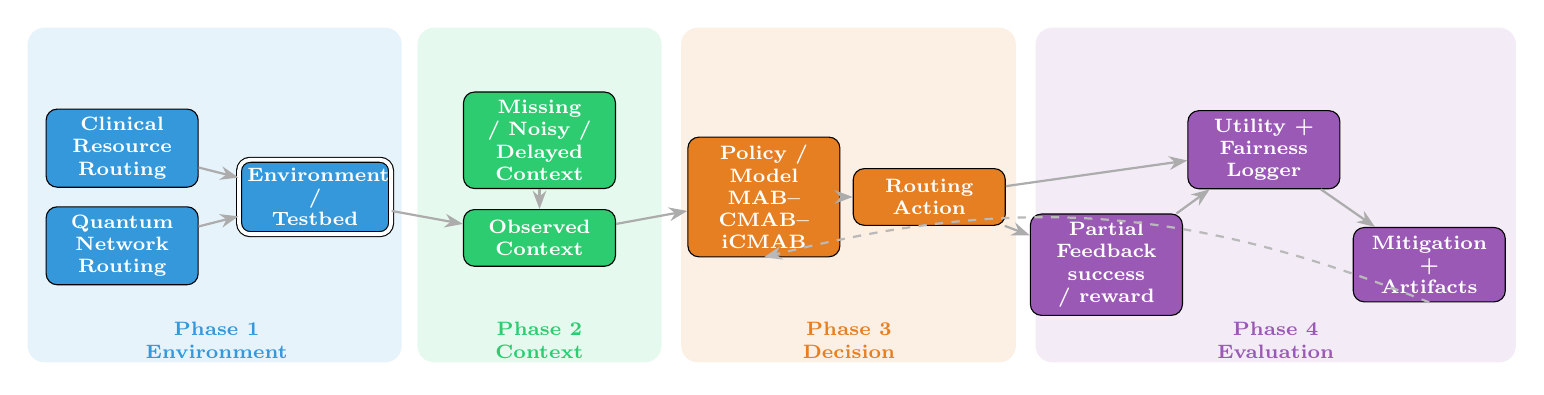
\begin{tikzpicture}[
  font=\scriptsize,
  phasebox/.style={draw, rounded corners=4pt, align=center,
              text width=1.72cm, minimum height=0.72cm,
              inner sep=3pt, text=white, font=\scriptsize\bfseries},
  phase1/.style={phasebox, fill=phase1blue},
  phase2/.style={phasebox, fill=phase2green},
  phase3/.style={phasebox, fill=phase3orange},
  phase4/.style={phasebox, fill=phase4purple},
  arr/.style={-Stealth, thick, gray!65},
  darr/.style={-Stealth, thick, dashed, gray!55},
  lbl/.style={font=\scriptsize\bfseries, align=center}
]
\fill[phase1blue!12, rounded corners=6pt]   (-0.65,-2.10) rectangle (4.10,2.15);
\fill[phase2green!12, rounded corners=6pt]  (4.30,-2.10) rectangle (7.40,2.15);
\fill[phase3orange!12, rounded corners=6pt] (7.65,-2.10) rectangle (11.90,2.15);
\fill[phase4purple!12, rounded corners=6pt] (12.15,-2.10) rectangle (18.25,2.15);

\node[phase1] (clin) at (0.55,0.62) {Clinical\\Resource Routing};
\node[phase1] (quant) at (0.55,-0.62) {Quantum\\Network Routing};
\node[phase1, double, double distance=1.4pt] (env) at (3.00,0.00) {Environment /\\Testbed};

\node[phase2] (deg) at (5.85,0.72) {Missing / Noisy /\\Delayed Context};
\node[phase2] (ctx) at (5.85,-0.52) {Observed\\Context};

\node[phase3] (pol) at (8.70,0.00) {Policy / Model\\MAB--CMAB--iCMAB};
\node[phase3] (act) at (10.80,0.00) {Routing\\Action};

\node[phase4] (fb)  at (13.05,-0.86) {Partial Feedback\\success / reward};
\node[phase4] (log) at (15.05,0.60) {Utility + Fairness\\Logger};
\node[phase4] (mit) at (17.15,-0.86) {Mitigation +\\Artifacts};

\draw[arr] (clin)--(env);
\draw[arr] (quant)--(env);
\draw[arr] (env)--(ctx);
\draw[arr] (deg)--(ctx);
\draw[arr] (ctx)--(pol);
\draw[arr] (pol)--(act);
\draw[arr] (act)--(fb);
\draw[arr] (act)--(log);
\draw[arr] (fb)--(log);
\draw[arr] (log)--(mit);
\draw[darr] (mit.south) to[bend right=18] (pol.south);

\node[lbl, text=phase1blue]   at (1.75,-1.82) {\textbf{Phase 1}\\Environment};
\node[lbl, text=phase2green]  at (5.85,-1.82) {\textbf{Phase 2}\\Context};
\node[lbl, text=phase3orange] at (9.78,-1.82) {\textbf{Phase 3}\\Decision};
\node[lbl, text=phase4purple] at (15.20,-1.82) {\textbf{Phase 4}\\Evaluation};
\end{tikzpicture}%
}

\vspace{0.45em}
\scriptsize
\begin{tabular}{p{0.22\textwidth}p{0.65\textwidth}}
\toprule
\textbf{Domain element} & \textbf{Current implementation mapping} \\
\midrule
Environment / testbed & \texttt{ClinicalEnvironment} plus preserved quantum-routing testbed path \\
Context observation & site/cohort/service context, missing-context flags, stale/noisy route information \\
Policy / action & \texttt{ClinicalModelRegistry}, \texttt{FairAllocatorV1}, \texttt{ClinicalBanditUCB}, MAB/CMAB/iCMAB routing policies \\
Evaluation / mitigation & partial feedback, \texttt{ClinicalEquitasMediator}, fairness states, summaries, manifests, figures \\
\bottomrule
\end{tabular}

\vspace{0.25em}
\begin{itemize}\scriptsize
  \item The model captures the shared SDS loop: only the chosen action creates observed feedback; unchosen actions remain counterfactual.
  \item Fairness risk appears when context quality is systematically worse for one group, site, cohort, or route class.
\end{itemize}
\end{frame}

\begin{frame}{Why the Domain Model Changed}
\begin{columns}[T]
\begin{column}{0.48\textwidth}
\centering
\textbf{Old domain view}

\vspace{0.3em}
\resizebox{\linewidth}{!}{%
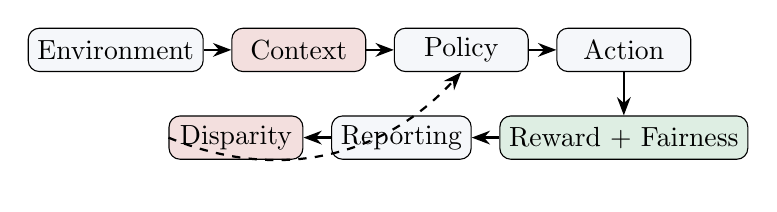
\begin{tikzpicture}[
  node distance=0.42cm,
  smallbox/.style={draw, rounded corners, align=center, minimum width=1.7cm, minimum height=0.55cm, fill=softgray},
  bad/.style={draw, rounded corners, align=center, minimum width=1.7cm, minimum height=0.55cm, fill=softred!18},
  good/.style={draw, rounded corners, align=center, minimum width=1.7cm, minimum height=0.55cm, fill=softgreen!18},
  arr/.style={-{Stealth}, thick}
]
\node[smallbox] (env) {Environment};
\node[bad, right=0.35cm of env] (ctx) {Context};
\node[smallbox, right=0.35cm of ctx] (pol) {Policy};
\node[smallbox, right=0.35cm of pol] (act) {Action};
\node[good, below=0.55cm of act] (out) {Reward + Fairness};
\node[smallbox, left=0.35cm of out] (rep) {Reporting};
\node[bad, left=0.35cm of rep] (harm) {Disparity};

\draw[arr] (env) -- (ctx);
\draw[arr] (ctx) -- (pol);
\draw[arr] (pol) -- (act);
\draw[arr] (act) -- (out);
\draw[arr] (out) -- (rep);
\draw[arr] (rep) -- (harm);
\draw[arr,dashed] (harm.west) to[bend right=35] (pol.south);
\end{tikzpicture}}
\vspace{0.35em}

{\scriptsize Compact pipeline, but some concepts were merged together.}
\end{column}

\begin{column}{0.48\textwidth}
\centering
\textbf{Updated domain view}

\vspace{0.3em}
\resizebox{\linewidth}{!}{%
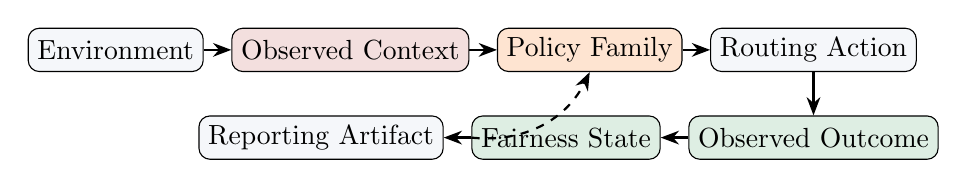
\begin{tikzpicture}[
  node distance=0.42cm,
  smallbox/.style={draw, rounded corners, align=center, minimum width=1.7cm, minimum height=0.55cm, fill=softgray},
  bad/.style={draw, rounded corners, align=center, minimum width=1.7cm, minimum height=0.55cm, fill=softred!18},
  good/.style={draw, rounded corners, align=center, minimum width=1.7cm, minimum height=0.55cm, fill=softgreen!18},
  orangebox/.style={draw, rounded corners, align=center, minimum width=1.7cm, minimum height=0.55cm, fill=ritorange!18},
  arr/.style={-{Stealth}, thick}
]
\node[smallbox] (env) {Environment};
\node[bad, right=0.35cm of env] (ctx) {Observed Context};
\node[orangebox, right=0.35cm of ctx] (pol) {Policy Family};
\node[smallbox, right=0.35cm of pol] (act) {Routing Action};
\node[good, below=0.55cm of act] (out) {Observed Outcome};
\node[good, left=0.35cm of out] (fair) {Fairness State};
\node[smallbox, left=0.35cm of fair] (rep) {Reporting Artifact};

\draw[arr] (env) -- (ctx);
\draw[arr] (ctx) -- (pol);
\draw[arr] (pol) -- (act);
\draw[arr] (act) -- (out);
\draw[arr] (out) -- (fair);
\draw[arr] (fair) -- (rep);
\draw[arr,dashed] (fair.west) to[bend right=35] (pol.south);
\end{tikzpicture}}
\vspace{0.35em}

{\scriptsize Clearer separation of decision, outcome, fairness audit, and reporting.}
\end{column}
\end{columns}

\vspace{0.6em}
\begin{block}{Why this matters}
\begin{itemize}
    \item The updated model separates \textbf{observed outcome} from \textbf{fairness state}, so fairness is treated as an audit layer rather than being hidden inside reward.
    \item It makes the \textbf{bandit setting} clearer: only the chosen action is observed, while the other actions remain \textbf{counterfactual}.
    \item It also makes the project more reproducible by showing that \textbf{reporting/validation artifacts} are explicit outputs of the framework.
\end{itemize}
\end{block}
\end{frame}

% Approach slides derived from DSCI601-Project_Proposal/approach_report/approach-writeup.tex.
% Keep this section aligned with the original approach report.

\begin{frame}{Approach Overview}
\begin{block}{Core approach from the approach report}
This project treats \textbf{clinical resource allocation} and \textbf{quantum-network routing} as structurally comparable routing problems. Both fail when a policy must allocate scarce resources while key context is missing, noisy, delayed, or excluded.
\end{block}

\vspace{0.4em}

\begin{columns}[T]
\begin{column}{0.48\textwidth}
\textbf{Clinical routing}
\begin{itemize}
    \item routes tests, retesting, and escalation follow-ups
    \item operates under incomplete or group-unequal patient context
    \item fairness risk appears as false-negative, delayed-care, or access gaps
\end{itemize}
\end{column}

\begin{column}{0.48\textwidth}
\textbf{Quantum routing}
\begin{itemize}
    \item routes entanglement and scarce qubit/link resources
    \item operates under noisy, stale, or partial network context
    \item fairness risk appears as service-quality gaps across flows
\end{itemize}
\end{column}
\end{columns}

\vspace{0.45em}
\begin{block}{Unifying claim}
The harmed groups or flows are often the ones whose context is missing, misrepresented, or not used correctly by the routing policy.
\end{block}
\end{frame}

\begin{frame}{Approach: Four-Phase Evaluation Model}
\centering
\resizebox{0.96\textwidth}{!}{%
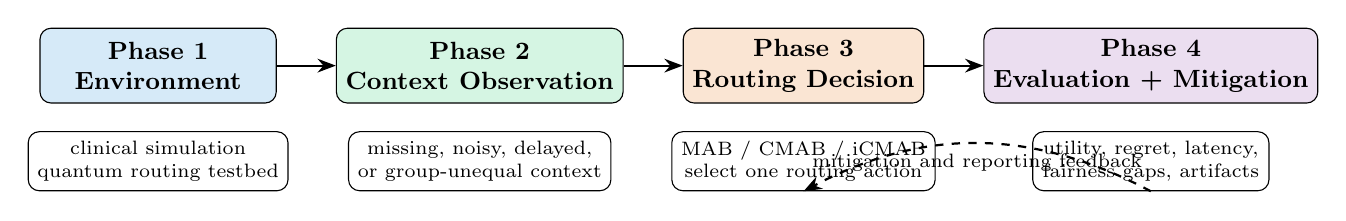
\begin{tikzpicture}[
  node distance=0.8cm,
  phase/.style={draw, rounded corners, align=center, minimum width=3.0cm, minimum height=0.95cm, font=\small\bfseries},
  detail/.style={draw, rounded corners, align=center, minimum width=3.0cm, minimum height=0.75cm, font=\scriptsize, fill=white},
  arr/.style={-{Stealth}, thick}
]

\node[phase, fill=phase1blue!20] (p1) {Phase 1\\Environment};
\node[phase, fill=phase2green!20, right=0.75cm of p1] (p2) {Phase 2\\Context Observation};
\node[phase, fill=phase3orange!20, right=0.75cm of p2] (p3) {Phase 3\\Routing Decision};
\node[phase, fill=phase4purple!20, right=0.75cm of p3] (p4) {Phase 4\\Evaluation + Mitigation};

\node[detail, below=0.35cm of p1] (d1) {clinical simulation\\quantum routing testbed};
\node[detail, below=0.35cm of p2] (d2) {missing, noisy, delayed,\\or group-unequal context};
\node[detail, below=0.35cm of p3] (d3) {MAB / CMAB / iCMAB\\select one routing action};
\node[detail, below=0.35cm of p4] (d4) {utility, regret, latency,\\fairness gaps, artifacts};

\draw[arr] (p1) -- (p2);
\draw[arr] (p2) -- (p3);
\draw[arr] (p3) -- (p4);
\draw[arr, dashed] (d4.south) to[bend right=28]
node[below, font=\scriptsize]{mitigation and reporting feedback} (d3.south);
\end{tikzpicture}
}

\vspace{0.55em}

\begin{block}{Why Phase 2 matters most}
The approach report identifies \textbf{Context Observation} as the root-cause phase: if context is missing or unreliable before the policy acts, routing disparities can compound even when the policy looks good on average.
\end{block}
\end{frame}

\begin{frame}{Approach: Why MAB, CMAB, and iCMAB}
\small
\begin{tabular}{p{0.20\textwidth}p{0.29\textwidth}p{0.39\textwidth}}
\toprule
\textbf{Policy level} & \textbf{What it sees} & \textbf{What it tests} \\
\midrule
\mab & action history only & What happens when the routing policy ignores context entirely. \\
\cmab & observed context & Whether available context improves utility and fairness, even when some context is incomplete or noisy. \\
\icmab & observed context plus informative or recovered context & Whether actively recovering or weighting missing context reduces disparity beyond standard contextual routing. \\
\bottomrule
\end{tabular}

\vspace{0.7em}

\begin{block}{Design rationale}
The policy spectrum directly tests the central research question: \textbf{how much routing harm is caused by missing context, and how much requires additional fairness mitigation?}
\end{block}
\end{frame}

\begin{frame}{Approach: Implementation and Evaluation Plan}
\small
\begin{tabular}{p{0.25\textwidth}p{0.34\textwidth}p{0.31\textwidth}}
\toprule
\textbf{Approach element} & \textbf{Implementation} & \textbf{Evaluation signal} \\
\midrule
Clinical testbed & simulation-first resource allocation with missing/noisy/group-unequal context & false-negative gaps, delayed-escalation gaps, allocation efficiency \\
Quantum testbed & existing quantum-routing environment with scarce links, qubits, and probabilistic success & success rate, latency, regret, service-equity gaps \\
Shared policy interface & MAB, CMAB, and iCMAB policies run across comparable decision records & utility--fairness tradeoff across context levels \\
Per-step logging & chosen action, observed feedback, group/flow state, fairness state, artifacts & when disparities emerge, persist, or reduce under mitigation \\
Mitigation layer & fairness-aware adjustment, EQUITAS-style mediation, or missingness-aware policy update & whether fairness evidence changes future routing decisions \\
\bottomrule
\end{tabular}

\vspace{0.6em}

\begin{block}{Main point}
The approach is not a late pivot. It is the original approach: a shared clinical--quantum bandit framework for testing whether better context leads to fairer and better routing.
\end{block}
\end{frame}


\begin{frame}{Updated Architecture Overview}
\centering
\vspace{-0.35em}
\resizebox{0.98\textwidth}{!}{%
% Self-contained architecture diagram for the DSCI601 final presentation.
% This file is intentionally safe to \input{} from main.tex.
% Compact vertical layout so the full diagram fits on one 16:9 slide.

\providecolor{phase1blue}{RGB}{52,152,219}
\providecolor{phase2green}{RGB}{46,204,113}
\providecolor{phase3orange}{RGB}{230,126,34}
\providecolor{phase4purple}{RGB}{155,89,182}

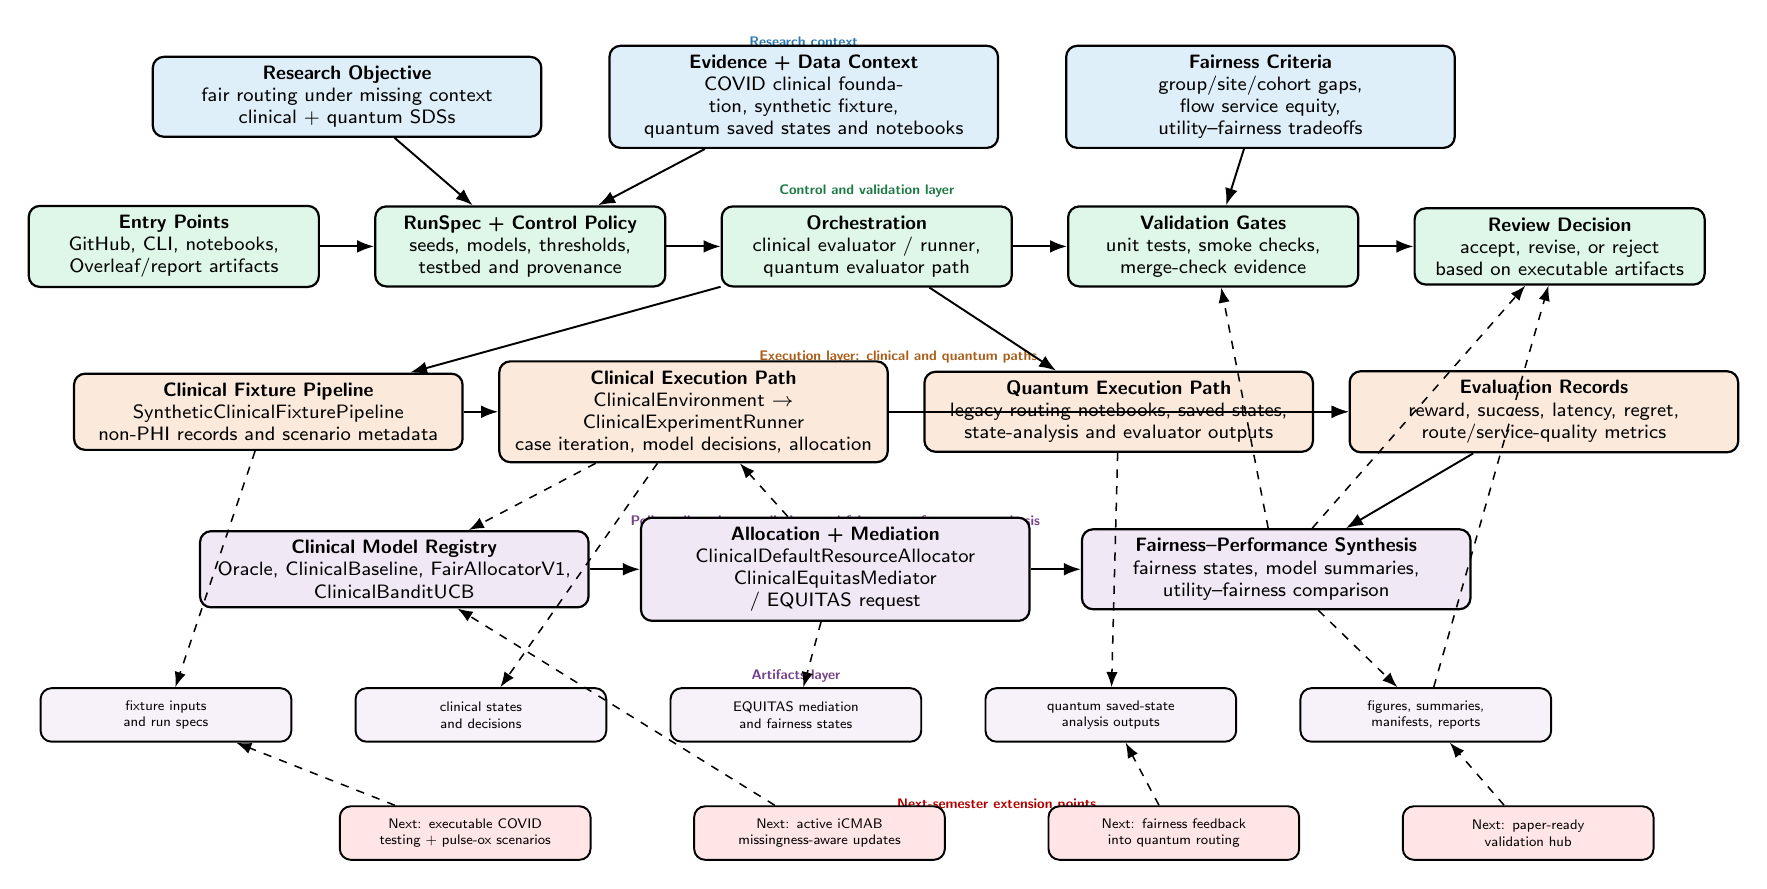
\begin{tikzpicture}[
font=\sffamily,
>=Latex,
layerlabel/.style={font=\sffamily\tiny\bfseries,align=center},
box/.style={rectangle,draw=black,rounded corners,minimum height=0.82cm,text width=3.45cm,align=center,fill=gray!8,line width=0.8pt,font=\sffamily\scriptsize},
widebox/.style={rectangle,draw=black,rounded corners,minimum height=0.88cm,text width=4.70cm,align=center,fill=gray!8,line width=0.8pt,font=\sffamily\scriptsize},
smallbox/.style={rectangle,draw=black,rounded corners,minimum height=0.68cm,text width=2.95cm,align=center,fill=gray!6,line width=0.7pt,font=\sffamily\tiny},
flow/.style={->,line width=0.70pt},
trace/.style={->,dashed,line width=0.55pt},
lab/.style={font=\sffamily\tiny,align=center}
]

% -------------------------------------------------------------------------
% Compact layer labels
% -------------------------------------------------------------------------
\node[layerlabel,text=phase1blue!80!black] at (5.8,6.95) {Research context};
\node[layerlabel,text=phase2green!60!black] at (6.6,5.05) {Control and validation layer};
\node[layerlabel,text=phase3orange!75!black] at (7.0,2.95) {Execution layer: clinical and quantum paths};
\node[layerlabel,text=phase4purple!75!black] at (6.2,0.85) {Policy, allocation, mediation, and fairness--performance synthesis};
\node[layerlabel,text=phase4purple!75!black] at (5.7,-1.10) {Artifacts layer};
\node[layerlabel,text=red!70!black] at (8.25,-2.75) {Next-semester extension points};

% -------------------------------------------------------------------------
% Top research context
% -------------------------------------------------------------------------
\node[widebox,fill=phase1blue!16] (objective) at (0,6.25)
{\textbf{Research Objective}\\fair routing under missing context\\clinical + quantum SDSs};

\node[widebox,fill=phase1blue!16] (evidence) at (5.8,6.25)
{\textbf{Evidence + Data Context}\\COVID clinical foundation, synthetic fixture,\\quantum saved states and notebooks};

\node[widebox,fill=phase1blue!16] (criteria) at (11.6,6.25)
{\textbf{Fairness Criteria}\\group/site/cohort gaps, flow service equity,\\utility--fairness tradeoffs};

% -------------------------------------------------------------------------
% Control layer
% -------------------------------------------------------------------------
\node[box,fill=phase2green!16] (entry) at (-2.2,4.35)
{\textbf{Entry Points}\\GitHub, CLI, notebooks,\\Overleaf/report artifacts};

\node[box,fill=phase2green!16] (runspec) at (2.2,4.35)
{\textbf{RunSpec + Control Policy}\\seeds, models, thresholds,\\testbed and provenance};

\node[box,fill=phase2green!16] (orchestration) at (6.6,4.35)
{\textbf{Orchestration}\\clinical evaluator / runner,\\quantum evaluator path};

\node[box,fill=phase2green!16] (validation) at (11.0,4.35)
{\textbf{Validation Gates}\\unit tests, smoke checks,\\merge-check evidence};

\node[box,fill=phase2green!16] (review) at (15.4,4.35)
{\textbf{Review Decision}\\accept, revise, or reject\\based on executable artifacts};

% -------------------------------------------------------------------------
% Execution layer
% -------------------------------------------------------------------------
\node[widebox,fill=phase3orange!16] (fixture) at (-1.0,2.25)
{\textbf{Clinical Fixture Pipeline}\\SyntheticClinicalFixturePipeline\\non-PHI records and scenario metadata};

\node[widebox,fill=phase3orange!16] (clinenv) at (4.4,2.25)
{\textbf{Clinical Execution Path}\\ClinicalEnvironment $\rightarrow$ ClinicalExperimentRunner\\case iteration, model decisions, allocation};

\node[widebox,fill=phase3orange!16] (quantum) at (9.8,2.25)
{\textbf{Quantum Execution Path}\\legacy routing notebooks, saved states,\\state-analysis and evaluator outputs};

\node[widebox,fill=phase3orange!16] (eval) at (15.2,2.25)
{\textbf{Evaluation Records}\\reward, success, latency, regret,\\route/service-quality metrics};

% -------------------------------------------------------------------------
% Policy and mediation layer
% -------------------------------------------------------------------------
\node[widebox,fill=phase4purple!14] (models) at (0.6,0.25)
{\textbf{Clinical Model Registry}\\Oracle, ClinicalBaseline, FairAllocatorV1,\\ClinicalBanditUCB};

\node[widebox,fill=phase4purple!14] (alloc) at (6.2,0.25)
{\textbf{Allocation + Mediation}\\ClinicalDefaultResourceAllocator\\ClinicalEquitasMediator / EQUITAS request};

\node[widebox,fill=phase4purple!14] (fair) at (11.8,0.25)
{\textbf{Fairness--Performance Synthesis}\\fairness states, model summaries,\\utility--fairness comparison};

% -------------------------------------------------------------------------
% Artifacts layer
% -------------------------------------------------------------------------
\node[smallbox,fill=phase4purple!8] (a1) at (-2.3,-1.60) {fixture inputs\\and run specs};
\node[smallbox,fill=phase4purple!8] (a2) at (1.7,-1.60) {clinical states\\and decisions};
\node[smallbox,fill=phase4purple!8] (a3) at (5.7,-1.60) {EQUITAS mediation\\and fairness states};
\node[smallbox,fill=phase4purple!8] (a4) at (9.7,-1.60) {quantum saved-state\\analysis outputs};
\node[smallbox,fill=phase4purple!8] (a5) at (13.7,-1.60) {figures, summaries,\\manifests, reports};

% -------------------------------------------------------------------------
% Next semester extension markers
% -------------------------------------------------------------------------
\node[smallbox,fill=red!10] (n1) at (1.5,-3.10) {Next: executable COVID\\testing + pulse-ox scenarios};
\node[smallbox,fill=red!10] (n2) at (6.0,-3.10) {Next: active iCMAB\\missingness-aware updates};
\node[smallbox,fill=red!10] (n3) at (10.5,-3.10) {Next: fairness feedback\\into quantum routing};
\node[smallbox,fill=red!10] (n4) at (15.0,-3.10) {Next: paper-ready\\validation hub};

% -------------------------------------------------------------------------
% Main flows
% -------------------------------------------------------------------------
\draw[flow] (objective) -- (runspec);
\draw[flow] (evidence) -- (runspec);
\draw[flow] (criteria) -- (validation);

\draw[flow] (entry) -- (runspec);
\draw[flow] (runspec) -- (orchestration);
\draw[flow] (orchestration) -- (validation);
\draw[flow] (validation) -- (review);

\draw[flow] (orchestration) -- (fixture);
\draw[flow] (fixture) -- (clinenv);
\draw[flow] (orchestration) -- (quantum);
\draw[flow] (clinenv) -- (eval);
\draw[flow] (quantum) -- (eval);

\draw[flow] (models) -- (alloc);
\draw[flow] (alloc) -- (fair);
\draw[flow] (eval) -- (fair);

% -------------------------------------------------------------------------
% Shorter trace flows
% -------------------------------------------------------------------------
\draw[trace] (clinenv) -- (models);
\draw[trace] (alloc) -- (clinenv);
\draw[trace] (fair) -- (validation);
\draw[trace] (fair) -- (review);

\draw[trace] (fixture) -- (a1);
\draw[trace] (clinenv) -- (a2);
\draw[trace] (alloc) -- (a3);
\draw[trace] (quantum) -- (a4);
\draw[trace] (fair) -- (a5);
\draw[trace] (a5) -- (review);

% Bottom extension arrows shortened by routing to closest artifact/policy anchors
\draw[trace] (n1) -- (a1);
\draw[trace] (n2) -- (models);
\draw[trace] (n3) -- (a4);
\draw[trace] (n4) -- (a5);

\end{tikzpicture}

}
\vspace{-0.15em}
\scriptsize
\textbf{Read left to right:} research context and evidence feed controlled runs; clinical and quantum execution paths produce evaluation records; allocation, EQUITAS mediation, and fairness--performance synthesis generate reviewable artifacts.
\end{frame}

\begin{frame}{What Changed in the Current Architecture}
\small
\begin{tabular}{p{0.24\textwidth}p{0.34\textwidth}p{0.32\textwidth}}
\toprule
\textbf{Region} & \textbf{Current implementation} & \textbf{Why it matters} \\
\midrule
Clinical execution path & \texttt{ClinicalEnvironment}, \texttt{ClinicalExperimentRunner}, \texttt{ClinicalExperimentEvaluator} & Clinical work is executable through a runner/evaluator path. \\
Policy/model path & \texttt{ClinicalModelRegistry}: Oracle, ClinicalBaseline, FairAllocatorV1, ClinicalBanditUCB & The deck can discuss actual model families rather than generic policy boxes. \\
Allocation + mediation & \texttt{ClinicalDefaultResourceAllocator} and \texttt{ClinicalEquitasMediator} & Fairness connects to allocation decisions through mediation, not only post-hoc reporting. \\
Quantum path & legacy quantum notebooks, saved states, state-analysis outputs & Existing quantum routing work remains preserved and feeds the same evaluation surface. \\
Artifacts layer & fairness states, summaries, figures, manifests, reports & The architecture produces evidence that can be reviewed, reproduced, and cited. \\
\bottomrule
\end{tabular}
\end{frame}

\begin{frame}{Architecture Layers in Detail}
\small
\begin{tabular}{p{0.22\textwidth}p{0.32\textwidth}p{0.36\textwidth}}
\toprule
\textbf{Layer} & \textbf{Key components} & \textbf{Responsibility} \\
\midrule
Control + validation & RunSpec, seeds, thresholds, smoke checks, merge criteria & control experiments and acceptance evidence \\
Execution & Clinical fixture, ClinicalEnvironment, quantum saved states & create decision settings and produce outcome records \\
Policy + allocation & ClinicalModelRegistry, FairAllocatorV1, ClinicalBanditUCB, allocator & choose routing actions under partial feedback \\
Mediation + synthesis & ClinicalEquitasMediator, fairness states, evaluator summaries & combine utility, fairness, and intervention context \\
Artifacts & figures, reports, manifests, state-analysis outputs & make results reproducible and reviewable \\
\bottomrule
\end{tabular}
\end{frame}

\begin{frame}{Preliminary Framework Results}
\begin{center}
\begin{tabular}{p{0.43\textwidth}p{0.42\textwidth}}
\toprule
Evidence item & Result \\
\midrule
Clinical embedded path & evaluator, runner, environment, allocator, models, and EQUITAS context run end-to-end \\
Clinical fairness smoke & 16 fairness states across four model families \\
Non-oracle efficiency & FairAllocatorV1: 91.23\%; ClinicalBanditUCB: 84.21\%; ClinicalBaseline: 75.09\% oracle efficiency \\
Reporting layer & 21 manifest-linked artifacts and model-stratified summaries \\
Quantum compatibility & legacy quantum path preserved with fairness sidecar artifacts \\
\bottomrule
\end{tabular}
\end{center}
\end{frame}

\begin{frame}{GitHub Code Review Break}
\begin{block}{Show 2--3 classes not used in the midterm}
Open GitHub and connect each class to the architecture diagram.
\end{block}
\small
\begin{tabular}{p{0.34\textwidth}p{0.48\textwidth}}
\toprule
Class / file to show & Architecture connection \\
\midrule
\texttt{ClinicalExperimentEvaluator} & evaluator orchestration, fairness states, artifacts \\
\texttt{ClinicalExperimentRunner} & run execution over seeds, models, and allocations \\
\texttt{ClinicalModelRegistry} & model families: Oracle, baseline, FairAllocatorV1, ClinicalBanditUCB \\
\texttt{equitas\_mediator.py} & mediation layer and fairness audit context \\
\bottomrule
\end{tabular}
\end{frame}

\begin{frame}{Working Demo Plan}
\begin{enumerate}
    \item Run the clinical fairness smoke/demo path.
    \item Show generated fairness states and model-stratified summaries.
    \item Show report artifacts and manifest linkage.
    \item Point to the COVID clinical foundation as the clinical evidence base.
    \item Explain how the quantum legacy path connects to the same fairness--performance layer.
\end{enumerate}
\end{frame}

\begin{frame}{Next Semester: Architecture Completion}
\begin{enumerate}
    \item Convert COVID test allocation and pulse-ox evidence into executable clinical environments.
    \item Complete active iCMAB missingness-aware updates.
    \item Close the loop so EQUITAS/fairness evidence updates future routing decisions.
    \item Add active fairness-adjusted quantum routing policies.
    \item Build a paper-ready validation hub linking claims, experiments, figures, and reproducibility metadata.
\end{enumerate}
\end{frame}

\begin{frame}{Takeaway}
\begin{block}{Main scientific claim}
Context quality is a fairness variable. Missing, ignored, or biased context can turn partial-feedback learning into repeated allocation harm.
\end{block}
\begin{block}{What was built}
A clinical--quantum evaluation framework that compares performance and fairness across the selected MAB spectrum while preserving reproducible artifacts.
\end{block}
\end{frame}

\begin{frame}{Selected References}
\scriptsize
\begin{itemize}
\item Sjoding et al. Racial bias in pulse oximetry measurement. \textit{New England Journal of Medicine}, 2020.
\item Fawzy et al. Pulse oximetry inaccuracy and delayed COVID treatment eligibility. \textit{JAMA Internal Medicine}, 2022.
\item Fawzy et al. Racial and ethnic discrepancy in pulse oximetry. \textit{JAMA Network Open}, 2023.
\item CDC/NCHS. COVID-19 provisional counts and health disparities.
\item DSCI601 workspace and project architecture materials.
\end{itemize}
\end{frame}

\end{document}
